\section{Bilan}

\paragraph{}
Finalement, \asmile{} fournit une offre complète d'intégration système autour des méthodes agiles et de l'intégration continue.
Le client peut suivre son projet avec Redmine, manipuler son code source avec Subversion tout en conservant un historique de l'ensemble des changements effectués, et enfin tester son application en continu avec Jenkins.
Il est accompagné par les ingénieurs système de \asmile{} qui peuvent lui proposer une prestation de conseil.

\paragraph{}
La \reffigure{pic:bilan} illustre une vue d'ensemble de l'offre.

\begin{figure}
	\centering
	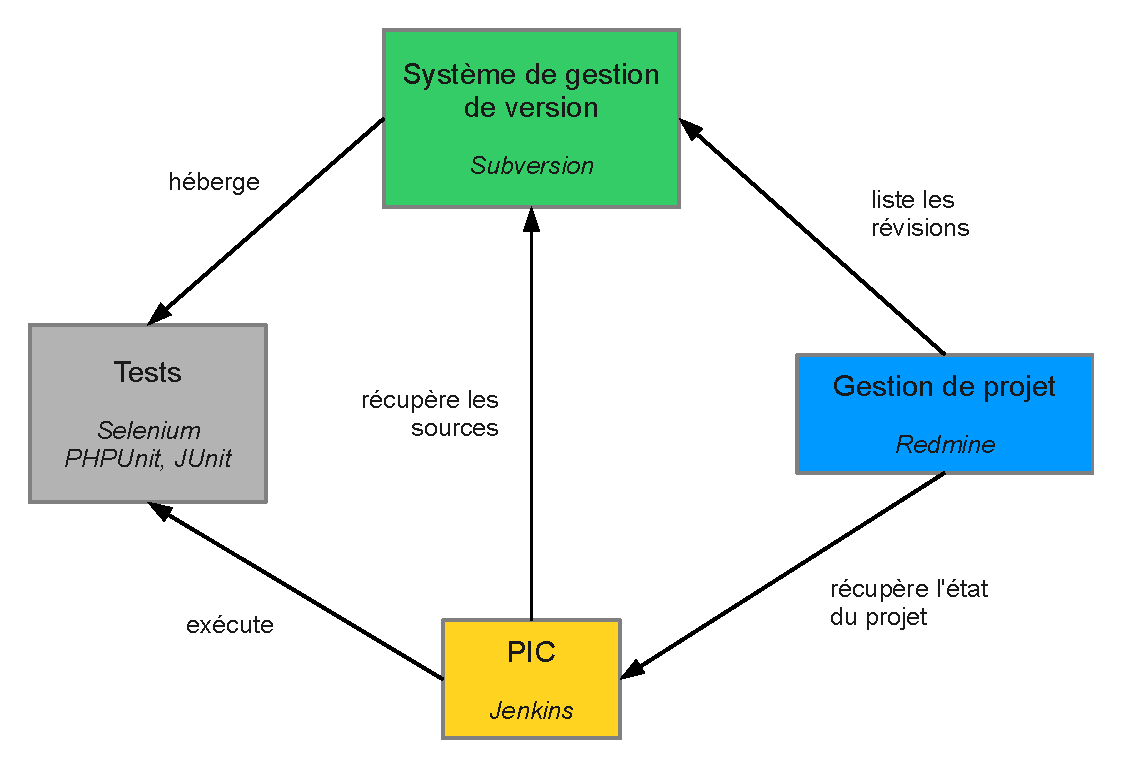
\includegraphics[width=14cm]{pic/bilan}
	\caption{Vue d'ensemble de l'offre \og Plateformes d'intégration continue \fg}
	\label{figure:pic:bilan}
\end{figure}

